\documentclass[11pt]{article}
\usepackage[utf8]{inputenc}
\usepackage[T1]{fontenc}
\usepackage{graphicx}
\usepackage{xcolor}
\usepackage{listings}
\usepackage{textcomp}
\usepackage[most]{tcolorbox}
%\usepackage{pythonhighlight}
\usepackage{minted}
%\usepackage{lscape}
\usepackage{rotating}
\usepackage{svg}
\usepackage[titletoc,title]{appendix}
\usepackage{animate}
\usepackage{subcaption}
%\usepackage{subfig;subfigure}
%\usepackage[dotinlabels]{titletoc}

%\usepackage[autostyle]{csquotes}

\usepackage[backend=bibtex,citestyle=authoryear,maxnames=1]{biblatex}
%\addbibresource{biblio.bib}
\bibliography{biblio.bib}

\newcommand{\source}[1]{\vspace*{-0.4cm}\caption*{\textit{Source: {#1}}}}
\renewcommand{\contentsname}{Table des matières}
\newcommand{\mycite}[1]{ (\cite{#1})}
\newcommand{\tocheck}[1]{\textcolor{lightgrey}{#1}}
\newcommand{\tool}{\emph{FragScape}}
\newcommand{\qgis}{\emph{QGIS}}
\newcommand{\grass}{\emph{GRASS}}
\newcommand{\myfigureref}[1]{Figure \ref{#1} : \hyperref[#1]{\nameref{#1}}\dotfill\pageref{#1}}
\newcommand{\meff}{taille effective de maille}
\newcommand{\Meff}{TODO}



\lstset{upquote=true,
    language=Python,
    showspaces=false,
    basicstyle=\small\ttfamily,
    %numbers=left,
    %numberstyle=\tiny,
    commentstyle=\color{gray}
    xleftmargin=1cm,
    % Code design
    identifierstyle=\color{editorGray},
    keywordstyle=[1]\color{editorBlue}\bfseries,
    keywordstyle=[2]\color{editorBlue}\bfseries,
    keywordstyle=[3]\color{editorBlack}\bfseries,
    keywordstyle=[4]\color{editorBlue}\bfseries,
    commentstyle=\color{editorGray}\ttfamily,
    stringstyle=\color{editorGreen}}

\definecolor{FunctionName}{rgb}{0,150,0}

% 2079971ms

\definecolor{editorLightGray}{cmyk}{0.05, 0.05, 0.05, 0.1}
\definecolor{editorWhite}{cmyk}{0, 0, 0, 0}
\definecolor{editorOrange}{cmyk}{0, 0.8, 1, 0}
\definecolor{editorBlue}{cmyk}{1, 0.6, 0, 0}
\definecolor{editorGreen}{rgb}{0, 0.5, 0}
\definecolor{editorGray}{rgb}{0.9,0.9,0.9}

%%novalidate

\usepackage{tikz}
\usepackage{calc}
\usepackage{booktabs}
\usepackage{datetime}


% colors
\definecolor{color1}{HTML}{000060}
%\definecolor{color1}{HTML}{8C260F}
\definecolor{color2}{HTML}{333333}
\definecolor{editorPurple}{cmyk}{0.45, 1, 0, 0}

% fonts
\usepackage{fontspec}
\defaultfontfeatures{Mapping=tex-text}
\setmainfont
[BoldFont=Lato-Bold.ttf,
ItalicFont=Lato-Italic.ttf,
BoldItalicFont=Lato-BoldItalic.ttf]
{Lato-Regular.ttf}
\newfontfamily\headingfont[ItalicFont=Lato-BlackItalic.ttf]{Lato-Black.ttf}
%%%

\usepackage{geometry}
\geometry{a4paper,
hmargin=20mm,vmargin=20mm,
head=0ex,foot=3ex}

\linespread{1.1}

\usepackage{caption}
\DeclareCaptionFormat{upper}{#1#2{#3}\par}
\captionsetup{labelfont={bf,color=color2},textfont={normalsize,color=color2},format = upper,figurename=FIGURE,tablename=TABLE}

%%% fancy sections
\usepackage{titlesec}
%\titleformat{\chapter}{\headingfont\LARGE\bfseries\scshape\color{color1}}{\thechapter}{1em}{}[\titlerule]
\titleformat{\section}{\color{color1}\headingfont\Large\bfseries\uppercase}{\thesection}{1em}{}[\titlerule]
\titleformat{\subsection}{\color{color1}\headingfont\large\bfseries\uppercase}{\thesubsection}{1em}{}
\titleformat{\subsubsection}{\color{color1}\headingfont\bfseries}{\thesubsubsection}{1em}{}

\setcounter{secnumdepth}{4}
\titleformat{\paragraph}{\color{color1}\headingfont\small\bfseries}{\theparagraph}{1em}{}
%\titlespacing*{\paragraph}
%{0pt}{3.25ex plus 1ex minus .2ex}{1.5ex plus .2ex}
%%%

\newdateformat{dateFormat}{%
\THEDAY/\THEMONTH/\THEYEAR}
\dateFormat

% head and foot
\usepackage{fancyhdr}

\pagestyle{fancy}
\lhead{}
\chead{}
\makeatletter
\rhead{}
%\rhead{\color{color2}\@date}
\makeatother
\newlength{\myheight}
\lfoot{\today
% \settoheight{\myheight}{\thepage}
% \raisebox{-2ex-0.5\myheight}{\includegraphics[height=4ex]{logo}}
}
\cfoot{\color{color2}TODO}
\rfoot{\color{color2}\thepage}
\renewcommand\headrulewidth{0pt}
\renewcommand\footrulewidth{0pt}

\fancypagestyle{style1}{
\fancyhf{}
\fancyfoot[L]{\color{lightgray} \textit{\today}}
\fancyfoot[C]{\color{lightgray} \textit{FragScape v1.0 - Notice d'utilisation}}
\fancyfoot[R]{\color{lightgray} \thepage / \pageref{LastPage}}
\renewcommand{\headrulewidth}{0pt}
}

\fancypagestyle{style2}{
\fancyhf{}
\fancyhead[C]{
\vspace{0.3cm}
\begin{tabular}{cccc}

\includegraphics[scale=0.07]{pictures/logoIrstea.png}\hspace{1cm}
&

\includegraphics[scale=0.2]{pictures/logoAgroParisTech.png}\hspace{1cm}
&

\includegraphics[scale=0.25]{pictures/logoTetis.png}\hspace{1cm}
&

\includegraphics[scale=0.9]{pictures/logoCRTVB.png}\hspace{1cm}
&

\includegraphics[scale=1.0]{pictures/logoMTES.png}
\end{tabular}
\renewcommand{\headrulewidth}{0pt}
}}

% custom titlepage
\makeatletter
\newcommand*\DefVar[1]{\@namedef{#1}##1{\global\@namedef{get#1}{##1}}}
\DefVar{summary}
%\vspace{4cm}
\renewcommand{\maketitle}{
\begin{center}
\begin{tabular}{ccc}

\includegraphics[scale=0.07]{pictures/logoIrstea.png}\hspace{1cm}
&

\includegraphics[scale=0.2]{pictures/logoAgroParisTech.png}
&

\includegraphics[scale=0.25]{pictures/logoTetis.png}
\end{tabular}

\vspace{1cm}

\begin{tabular}{lr}

\includegraphics[scale=0.9]{pictures/logoCRTVB.png}\hspace{1cm}
&

\includegraphics[scale=1.0]{pictures/logoMTES.png}
\end{tabular}
\vspace{2cm}

{\color{color1}\headingfont\bfseries\huge
FragScape v1.0}

\vspace{1cm}

{\color{color1}\headingfont\bfseries\LARGE
Notice d'utilisation}

\vspace{1cm}

\today

\vspace{1cm}

{\fontsize{12}{15}\textnormal{
Mathieu Chailloux (IRSTEA / UMR TETIS) - \textit{mathieu.chailloux@irstea.fr}\\
Jennifer Amsallem (IRSTEA / UMR TETIS) - \textit{jennifer.amsallem@irstea.fr}\\
Jean-Pierre Chéry (AgroParisTech / UMR TETIS) - \textit{jean-pierre.chery@teledection.fr}\\
\bigskip
}}


%\headingfont\bfseries\Large\@author\par
%\bigskip\medskip
%\textit{\textnormal{Commanditaire :}}\\
%Pierre-Olaf Schut (UPEM) - {\fontsize{15}{18}\textnormal{po.schut@u-pem.fr}}
%{\color{color2}\normalfont\normalsize\textbf{Summary:}\\
%\getsummary}
\end{center}
\clearpage
}
\makeatother
%%%

%%% fancy boxes
\usepackage{tcolorbox}
\usepackage{wrapfig}
\def\fullboxbegin{
\bigskip
\begin{tcolorbox}[colback=color1,colframe=color1,coltext=white,arc=0mm,boxrule=0pt]
}
\def\fullboxend{\end{tcolorbox}\medskip}
%
\def\leftboxbegin{
\begin{wrapfigure}{l}{0.5\textwidth}
\begin{tcolorbox}[colback=color1,colframe=color1,coltext=white,arc=0mm,boxrule=0pt]
}
\def\leftboxend{
\end{tcolorbox}
\end{wrapfigure}
}
%
\def\rightboxbegin{
\begin{wrapfigure}{r}{0.5\textwidth}
\begin{tcolorbox}[colback=color1,colframe=color1,coltext=white,arc=0mm,boxrule=0pt]
}
\def\rightboxend{
\end{tcolorbox}
\end{wrapfigure}
}
%
\newcounter{frames}
\def\frameboxbegin#1{
\bigskip
\refstepcounter{frames}
\begin{tcolorbox}[colback=white,colframe=color1,arc=0mm,title={{\textbf{Encart \arabic{frames}} : #1}}]
}
\def\frameboxend{
\end{tcolorbox}
}
%%%


\usepackage{lipsum}
\usepackage{arydshln}
\usepackage{hyperref}

\usepackage{fancyhdr}
\usepackage{lastpage}

\usepackage{indentfirst}

\pagestyle{fancy}
\fancyhf{}

\setlength{\headsep}{1.3in}
\setlength{\voffset}{-30pt}
\setlength\parindent{0pt}


\let\tempone\itemize
\let\temptwo\enditemize
\renewenvironment{itemize}{\tempone\addtolength{\itemsep}{-0.5\baselineskip}}{\temptwo}
\renewenvironment{enumerate}{\tempone\addtolength{\itemsep}{-0.5\baselineskip}}{\temptwo}


%%%%%%%%%%%%%%%
% Title Page
\bigskip
%\title{Développement d'un plugin \emph{QGIS} pour modéliser les déplacements de la faune par la méthode de perméabilité des milieux pour la cartographie des continuités écologiques}
%\title{Titre quand meme plus court sinon c'est relou}
\bigskip

\date{\today}
%\summary{}
%%%%%%%%%%%%%%%

\begin{document}

\renewcommand{\appendixtocname}{Annexes}
\renewcommand{\appendixpagename}{\color{color1}{Annexes}} 
\sloppy

%\pagestyle{style2}

\vspace{4cm}

\maketitle

\clearpage

\pagestyle{style1}

\setlength{\headsep}{0.9in}

\tableofcontents

\hspace{4cm}

%\section*{Table des figures}


%\myfigureref{biogeoFragm}


%\pagebreak

%\section*{Table des figures}

\pagebreak

\section{Aperçu}

\tool\ est un plugin \qgis\ permettant de calculer les indicateurs de fragmentation du paysage définis dans l'article « Landscape division, splitting index, and effective mesh size: new measures of landscape fragmentation » \mycite{jaeger}.
Parmi ces indicateurs, la taille effective de maille est très largement utilisée pour quantifier la fragmentation du paysage. \tool\ définit une procédure en 4 étapes depuis les données brutes jusqu'au calcul des indicateurs et permet de sauvegarder la configuration de l'outil afin de pouvoir reproduire les résultats.

\subsection{Indicateurs de fragmentation du paysage}
\label{sec:metrics}

Jaeger définit dans son article\mycite{jaeger} trois nouvelles mesures de fragmentation du paysage :
\begin{itemize}
    \item le degré de fragmentation du paysage 
    \item le nombre effectif de mailles
    \item la taille effective de maille
\end{itemize}

Pour calculer ces indicateurs, les éléments du paysage considérés comme fragmentants sont retirés. Les éléments restants sont appelés « patchs ». Le paysage est alors composé de $n$ patchs. La superficie d'un patch est notée  $A_i$ avec $1 \leq i \leq n$. La superficie totale du territoire d'étude est notée $A_t$.

\subsubsection{Degré de fragmentation du paysage}

Le degré de cohérence ($C$), une mesure auxiliaire, est défini comme la probabilité que deux points choisis aléatoirement dans le territoire soient connectés (c.à.d. non séparés par des éléments fragmentants comme des routes ou des zones urbaines).

Le degré de fragmentation du paysage ($D$) est défini comme la probabilité que deux points choisis aléatoirement dans le territoire ne soient $pas$ connectés.

\hspace*{-0.5cm}
\begin{minipage}[c][1cm]{.46\linewidth}
\begin{align*}
C = \sum_{i=1}^{n}(\frac{A_{i}}{A_{t}})^{²}
\end{align*}
\end{minipage}
\begin{minipage}[c][1cm]{.46\linewidth}
\begin{align*}
D = 1 - C
\end{align*}
\end{minipage}

\subsubsection{Nombre effectif de mailles}

Le nombre effectif de mailles ($S$) est défini comme le nombre de patchs obtenu en découpant la superficie totale du territoire par une maille régulière de telle façon que la nouvelle configuration mène au même degré de fragmentation que la configuration initiale :
\begin{align*}
S = \frac{A_{t}^{2}}{\sum_{i=1}^{n}A_{i}^{2}}
\end{align*}

$S$ peut être interprété comme le nombre effectif de maille effectif d'un réseau avec une taille de maille constante divisant le territoire en $S$ patchs de taille $A_{t} / S$.

\subsubsection{Taille effective de maille}

La taille effective de maille ($m$) correspond à la taille des patchs quand le territoire est divisé en $S$ patchs (chacun de même taille $At/S$) avec le même degré de fragmentation que la configuration initiale :
\begin{align*}
m = \frac{A_{t}}{S} = \frac{1}{A_{t}}\sum_{i=1}^{n}A_{i}^{2}
\end{align*}

La densité de mailles ($s$) correspond au nombre de mailles par unité de surface.
Le produit net ($N$) est défini comme le produit de la taille effective de maille $m$ par la superficie totale du territoire.

\hspace*{-0.5cm}
\begin{minipage}[c][1cm]{.46\linewidth}
\begin{align*}
s = \frac{S}{A_{t}} = \frac{A_{t}}{\sum_{i=1}^{n}A_{i}^{2}} = \frac{1}{m}
\end{align*}
\end{minipage}
\begin{minipage}[c][1cm]{.46\linewidth}
\begin{align*}
N = m.{A_{t}} = \sum_{i=1}^{n}A_{i}^{2}
\end{align*}
\end{minipage}

%$S = \frac{S}{A_{t}} = \frac{A_{t}}{\sum_{i=1}^{n}A_{i}^{2}} = \frac{A_{t}}{S}$

%Le produit net ($N$) est défini comme le prorduit de la taille effective de maille $m$ par la superficie totale du territoire : $\frac{1}{A_{t}}\sum_{i=1}^{n}A_{i}^{2}$



\subsubsection{Méthode « Cross-Boundary Connection » (CBC)}
\label{sec:cbc}

Comme d'autres indicateurs du paysage basés sur la notion de patch, les indicateurs définis ci-dessus peuvent être biaisés car les limites du territoire sont considérées comme fragmentantes et peuvent ainsi artificiellement découper les patchs. Pour répondre à ce problème, l'article « Modification of the effective mesh size for measuring landscape fragmentation to solve the boundary problem »\mycite{moser} propose une nouvelle méthode de calcul.

Cette méthodes, appelée \textit{cross-boundary connections} (CBC), inclut la superficie des patchs à l'extérieur des « frontières » du territoire. La superficie totale d'un patch est notée $A_{i}^{cmpl}$. La somme de la superficie des patchs est notée $A_{total}^{cmpl}$. La formule de la taille effective de maille d'après la méthode CBC est alors :
\begin{align*}
m = \frac{1}{A_{t}}\sum_{i=1}^{n}A_{i}.A_{i}^{cmpl}
\end{align*}

Les autres indicateurs sont adaptés à la méthode CBC, ainsi les expressions $\sum_{i=1}^{n}A_{i}^{2}$ et $A_{t}^{2}$ sont respectivement remplacéees par les expressions $\sum_{i=1}^{n}A_{i}.A_{i}^{cmpl}$ et $A_{t}.A_{total}^{cmpl}$.

\subsection{Installation}

\tool\ est un plugin \qgis. \tool\ a été testé sur différents systèmes d'exploitation : Ubuntu bionic, Windows 10 et macOS Sierra.

\frameboxbegin{Prérequis}
\textbf{\color{red}La version de \qgis\ doit être supérieure ou égale à 3.4.0.}
\frameboxend

Pour installer \tool, ouvrir \qgis:
\begin{enumerate}
    \item aller dans le menu \texttt{Extension}
    \item ouvrir la fenêtre \texttt{Installer/Gérer les extensions}
    \item aller dans l'onglet \texttt{Paramètres} et vérifier que l'option \texttt{Montrer les extensions expérimentales} est cochée
    \item retourner dans l'onglet \texttt{Toutes}, taper \tool\ dans la barre de recherche, sélectionner le résultat et appuyer sur le bouton \texttt{Installer le plugin}
\end{enumerate}

Une fois installé, l'icône \includesvg{pictures/vector_grid.svg} de \tool\ devrait appraître dans la barre d'outils de QGIS.

Si ce n'est pas le cas, aller dans le menu \texttt{Extension} et une entrée \tool\ devrait être présente.

Si ce n'est toujours pas le cas, l'installation a échoué. Vérifier les messages d'erreur ou contacter l'équipe de support.

\subsection{Interface graphique}

La figure \ref{fig:paramsTab} montre un aperçu de l'interface de \tool. Elle est composée de 4 prinicpaux éléments :
\begin{itemize}
    \item la barre d'outils en haut : chargement/enregistrement de la configuration, changement de langue 
    \item le panneau d'aide à droite : description de l'étape courante
    \item la barre de progression en bas : avancée du traitement en cours
    \item le fenêtre principale : contenu de l'étape courante
\end{itemize}

\begin{figure}[h!]
    \centering
    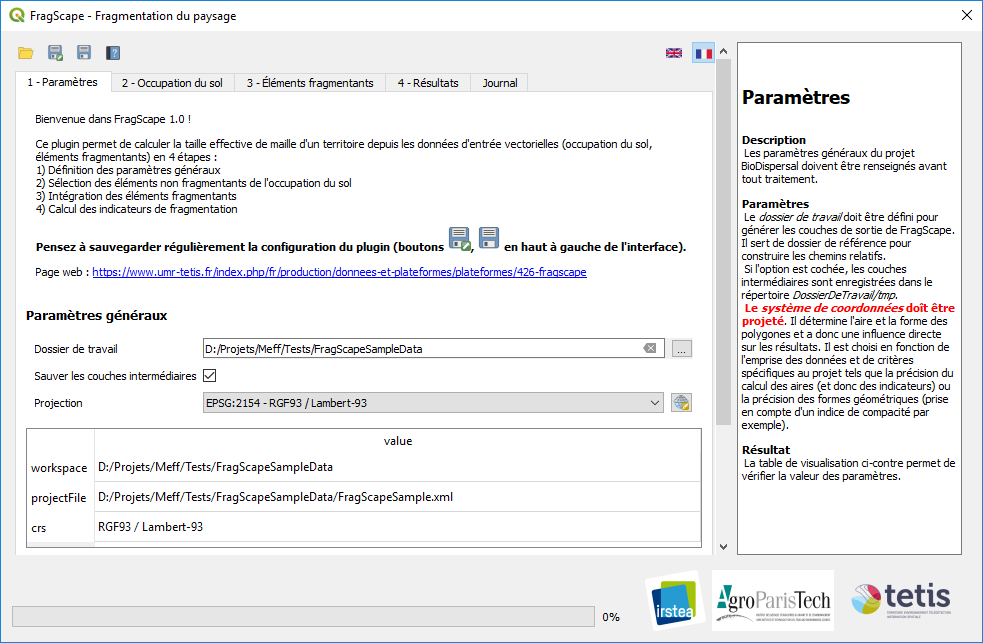
\includegraphics[scale=0.7]{pictures/paramsTabFr.png}
    \caption{Interface graphique de \tool\ v1.0}
    \label{fig:paramsTab}
    %\source{\tool\ v1.0}
\end{figure}

Dans la fenêtre principale, l'étape courante peut être composée de :
\begin{itemize}
    \item paramètres à renseigner (\texttt{Dossier de travail} par exemple)
    \item une table de visualisation permettant de vérifier la valeur actuelle des paramètres
    \item des boutons d'action (\texttt{Lancer la sélection} par exemple)
\end{itemize}

\section{Étapes}

\tool\ définit une procédure en 4 étapes depuis les données brutes jusqu'au calcul des indicateurs.

\subsection{Paramètres}

La première étape est de définir les paramètres globaux du projet \tool\ courant.

Le \texttt{Dossier de travail} doit être renseigné avec tout traitement car il définit le répertoire de sortie de \tool. Le résultat de chaque étape est stocké dans \textit{DossierDeTravail/outputs}. Attention au choix du dossier de travail car les fichiers déjà produits par \tool\ dans ce répertoire seront effacés.

Si l'option \texttt{Sauver les couches intermédiaires} est cochée, les couches intermédiaires sont enregistrées dans le répertoire \textit{DossierDeTravail/tmp}. Sinon, elles sont stockées dans le répertoire de traitements temporaire \qgis\ (le chemin est indiqué lors de sa création dans le journal).

La \texttt{Projection} est un système de projection cartographique qui doit être \textbf{métrique} et choisi en fonction de l'emprise des données. Il définit notammenet la forme et la superficie des entités.

\pagebreak

\subsection{Occupation du sol}

La deuxième étape est de sélectionner les éléments de l'occupation du sol considérés comme non-fragmentants.

Pour ce faire:
\begin{enumerate}
    \item Sélection la couche d'occupation du sol (paramètre \texttt{Couche d'entrée}).
    \item Si besoin, cocher l'option \texttt{Couper les données d'entrée} et choisir la \texttt{Couche de découpage}.
    \item Choisir le \texttt{Mode de sélection}.
    \item Renseigner les critères de sélection (champs ou expression).
    \item Appuyer sur le bouton \texttt{Lancer la sélection}.
\end{enumerate}
\hspace*{-0.5cm}
En mode \texttt{Par valeur de champ}, la sélection s'effectue ainsi :
\hspace*{-0.5cm}
\begin{itemize}
    \item Choisir le \texttt{Champ de sélection}, le champ contenant la classe d'occupation du sol (par exemple \textit{CODE\_2012} pour les données Corine Land Cover 2012).
    \item Il est possible de choisir un \texttt{Champ de description} contenant la description des classes d'occupation du sol pour plus de clarté. Cette étape est optionnelle.
    \item Appuyer sur le bouton \texttt{Afficher les valeurs de champ}.
    \item Cocher les classes d'occupation du sol à sélectionner dans la colonne \texttt{toSelect} de la table.
\end{itemize}

En mode \texttt{Par expression}, la sélection est réalisée en renseignant une expression booléenne (c.à.d. pouvant être évaluée comme vraie ou fausse). Les entités vérifiant cette expression sont sélectionnées. Si l'expression est vide, toutes les entités sont sélectionnées.

La figure \ref{fig:landuseTab} montre un exemple d'utilisation de l'interface de sélection de l'occupation du sol.

\begin{figure}[h!]
    \centering
    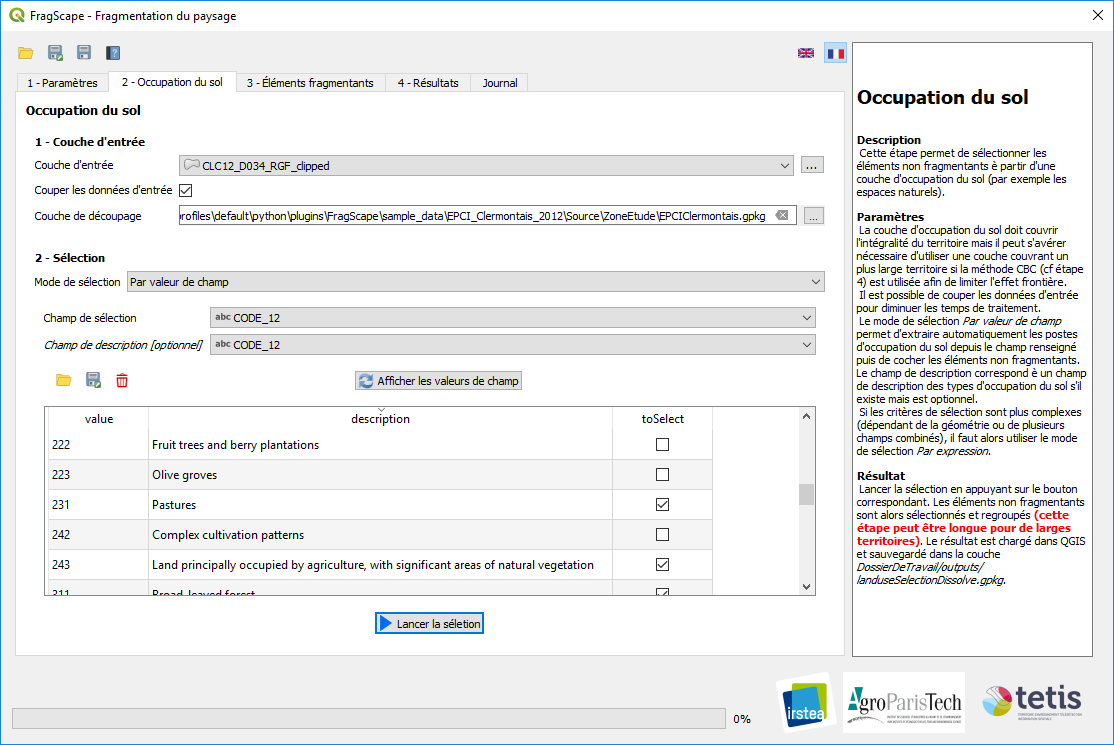
\includegraphics[scale=0.6]{pictures/landuseTabFr.png}
    \caption{Onglet \textit{Occupation du sol} de \tool\ v1.0}
    \label{fig:landuseTab}
    %\source{\tool\ v1.0}
\end{figure}

\subsection{Fragmentation}

La troisième étape est de sélectionner les éléments fragmentants.

Pour chaque type de fragmentation, il faut:
\begin{enumerate}
    \item Sélectionner la \texttt{Couche d'entrée} contenant les éléments de fragmentation ($roads.gpkg$ par exemple)
    \item Si besoin, sélectionner l'option \texttt{Couper les données d'entrée} et choisir une \texttt{Couche de découpage}.
    \item Si besoin, renseigner une \texttt{Expression} booléenne. Les entités vérifiant cette expression seront sélectionnées. Si l'expression est vide, toutes les entités sont sélectionnées. L'expression doit être construite depuis le widget \includesvg{pictures/mIconExpression.svg}.
    \item Renseigner une expression numérique définissant la zone \texttt{Tampon}. Obligatoire pour les données ponctuelles et linéaires. L'expression peut être variable et construite depuis le widget \includesvg{pictures/mIconExpression.svg}.
    \item Renseigner un \texttt{Identifiant} (unique dans le projet) pour ce type de fragmentation.
    \item Appuyer sur le bouton \texttt{Enregistrer la sélection}. La sélection renseignée apparaît alors comme un nouvelle ligne dans la table de visualisation.
\end{enumerate}

Une fois tous les éléments fragmentants renseignés, appuyer sur le bouton \texttt{Intégrer les éléments fragmentants}. Pour chaque sélection, les données sont sélectionnées et la zone tampon est appliquée. Les couches ainsi obtenues sont alors fusionnées et le résultat de cette fusion est utilisé pour calculer la différence avec la couche d'occupation du sol (l'intersection est supprimée). Enfin, cette différence est convertie en géométrie simple.

La couche finale produite par ces traitements est chargée dans QGIS et sauvegardé dans le fichier $Workspace/outputs/landuseFragmSingleGeom.gpkg$.

\begin{figure}[h!]
    \centering
    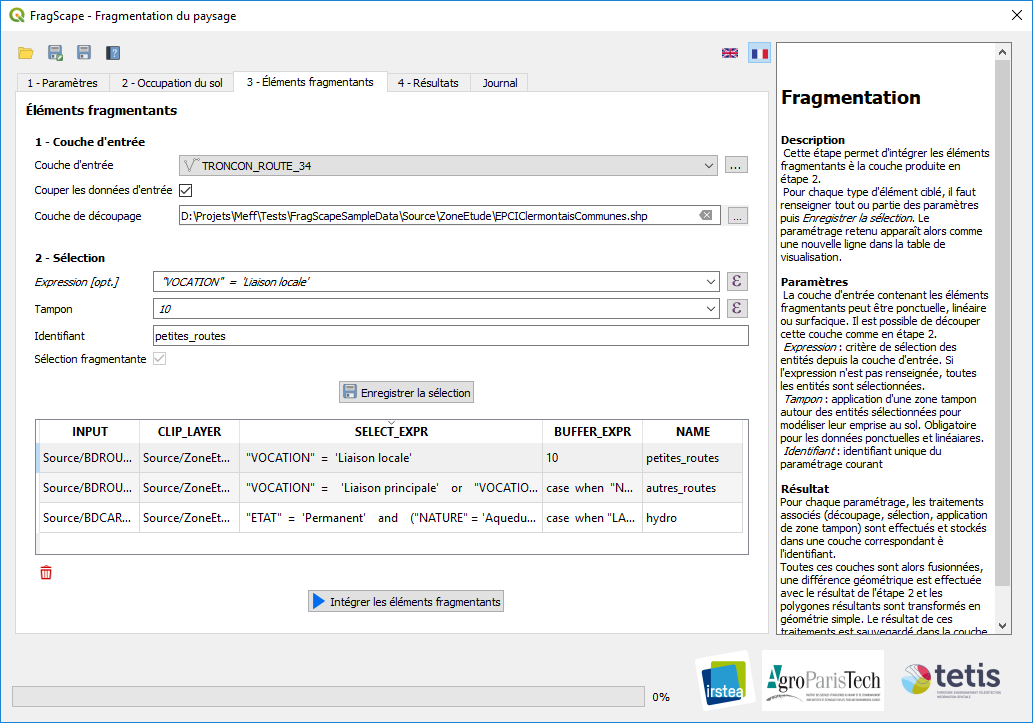
\includegraphics[scale=0.6]{pictures/fragmTabFr.png}
    \caption{Onglet \textit{Eléments fragmentants} de \tool\ v1.0}
    \label{fig:fragmTab}
    %\source{\tool\ v1.0}
\end{figure}

\subsection{Résultats}

La quatrième étape est le calcul des indicateurs de fragmentation

Pour ce faire:
\begin{itemize}
    \item Si besoin, \texttt{Filtrer les patchs} en renseignant une expression booléenne (basée sur la superficie par exemple)
    \item Renseigner la \texttt{Couche de rapportage}. Les indicateurs sont calculés pour chaque unité de rapportage. Pour calculer les indicateurs sur l'ensemble du territoire, la couche de rapportage doit ne contenir qu'une seule entité.
    \item Sélectionner la \texttt{Méthode de découpage} (cf section \ref{sec:cbc})
    \item Renseigner la \texttt{Couche de sortie}. Si la couche n'est pas reseignée, une couche mémoire est créée.
    \item Sélectionner l'\texttt{Unité de surface} (du mètre carré au kilomètre carré).
    \item Appuyer sur le bouton \texttt{Calculer les idicateurs}.
\end{itemize}

\begin{figure}[h!]
    \centering
    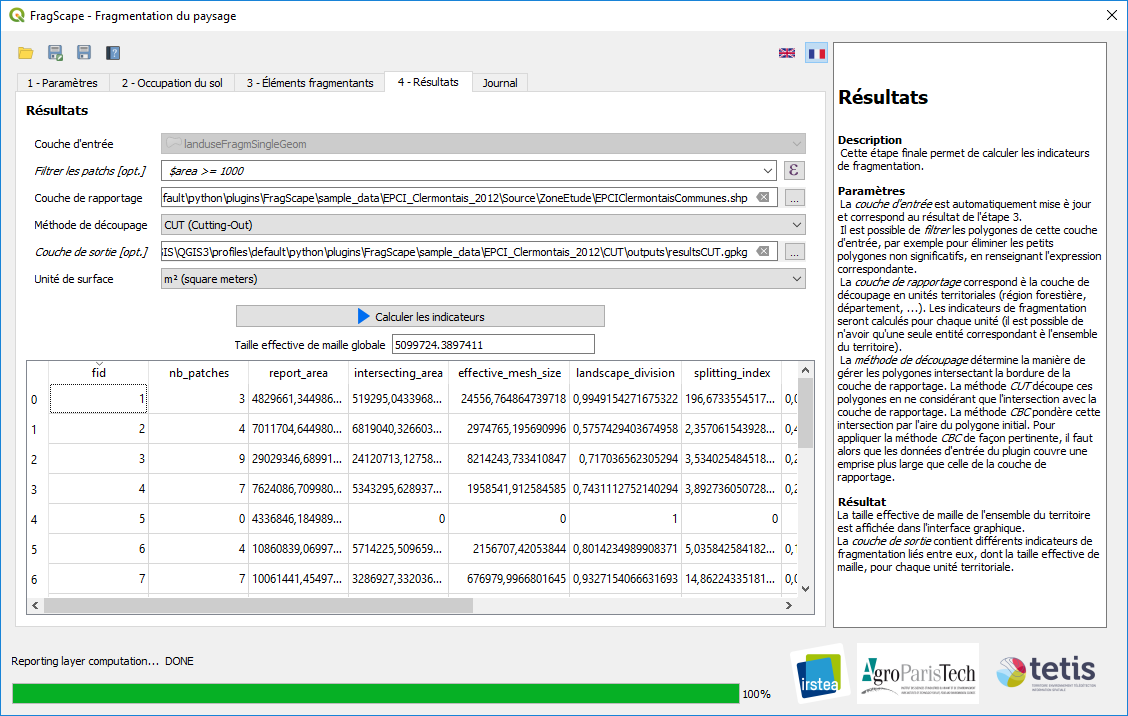
\includegraphics[scale=0.6]{pictures/resultsTabFr.png}
    \caption{Onglet \textit{Résultats} de \tool\ v1.0}
    \label{fig:resultsTab}
    %\source{\tool\ v1.0}
\end{figure}


La figure \ref{fig:resultsTab} montre l'interface de cette dernière étape.
Une fois les indicateurs calculés, la couche de sortie est chargée dans la table de visualisation et la taille effective de maille globale (sur l'ensemble du territoire) est affichée.
La couche de sortie contient un champ pour chaque métrique définie en section \ref{sec:metrics} plus de nouveaux champs :
\begin{itemize}
    \item \texttt{nb\_patches}: le nombre de patchs intersectant l'unité de rapportage
    \item \texttt{report\_area}: l'aire de l'unité de rapportage
    \item \texttt{intersecting\_area}: l'aire de l'intersection entre les patchs et l'unité de rapportage
    \item \texttt{layer/path}: couche temporaire contenant l'unité de rapportage initiale
\end{itemize}

\pagebreak

\section{Exemple}

Cette section montre un cas d'utilisation de \tool\ basé sur les données d'exemple (fournies avec le plugin dans le répertoire \href{https://github.com/MathieuChailloux/FragScape/tree/master/sample_data/EPCI_Clermontais_2012}{\texttt{sample\_data}}).

\begin{figure}[h!]
\centering
   \begin{subfigure}[b]{.48\textwidth}
      \includegraphics[width=\textwidth]{pictures/landuseInput.png}
      %\includegraphics[width=\textwidth]{pictures/CBC/landuseInput.png}
      \caption{Occupation du sol initiale}
   \end{subfigure}
   \begin{subfigure}[b]{.48\textwidth}
      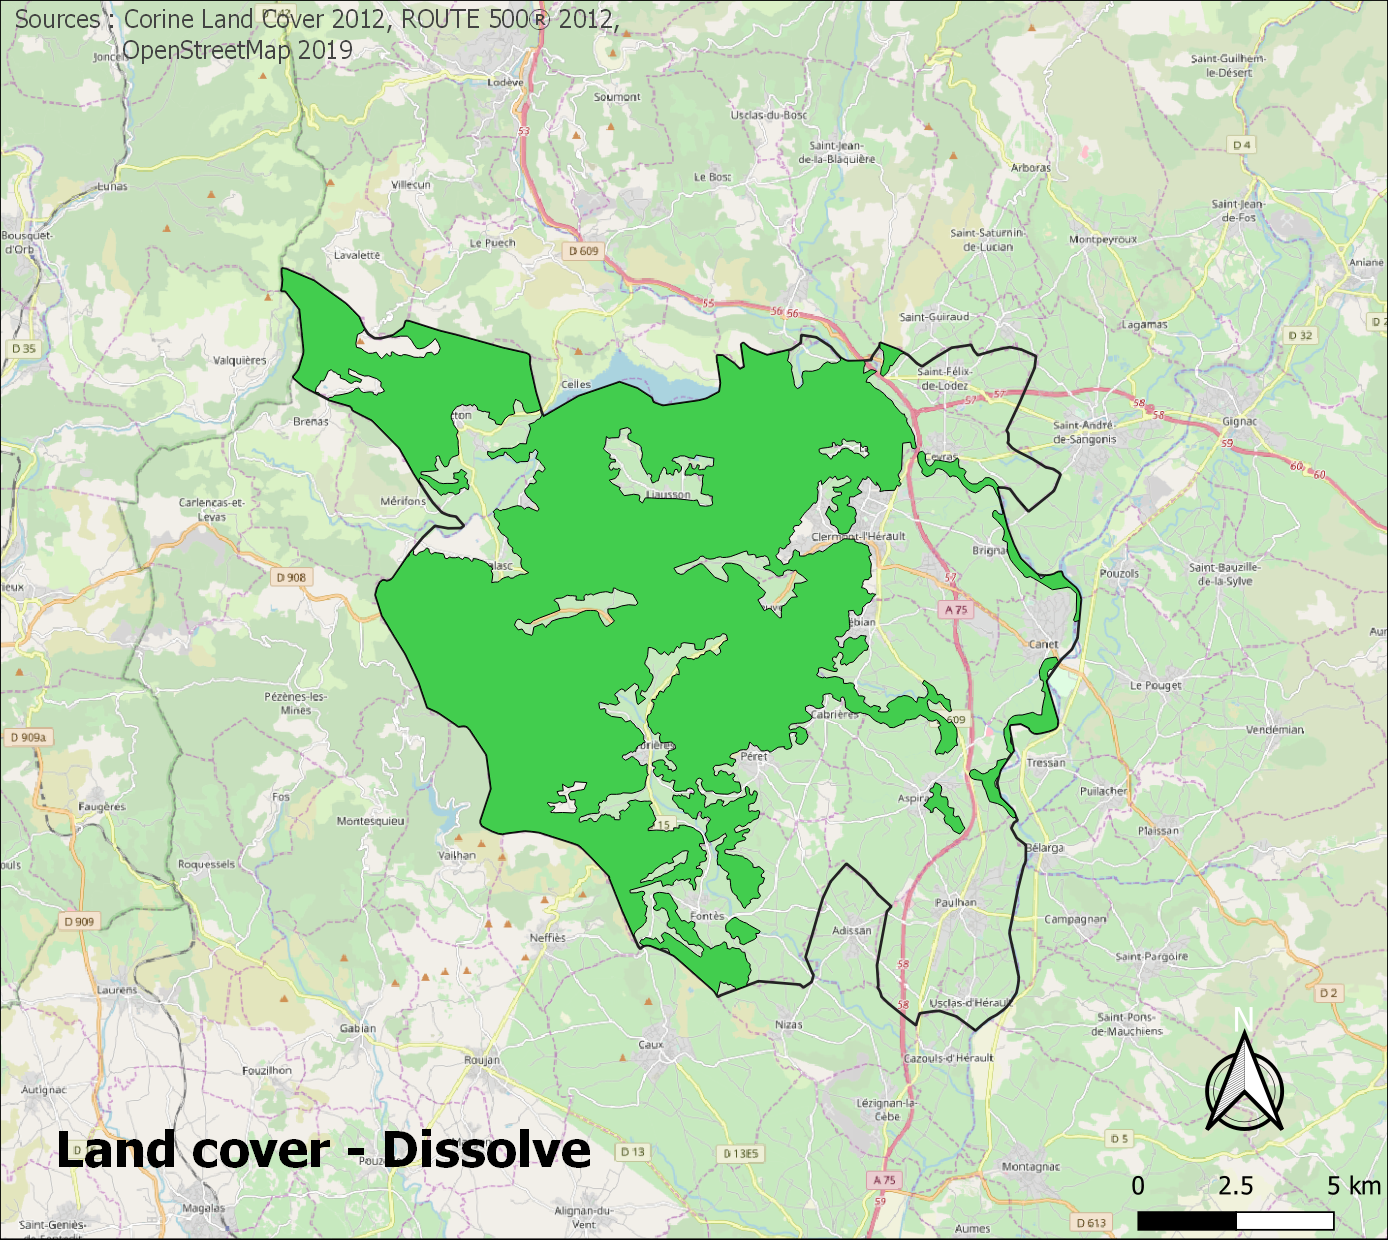
\includegraphics[width=\textwidth]{pictures/landuseDissolve.png}
      %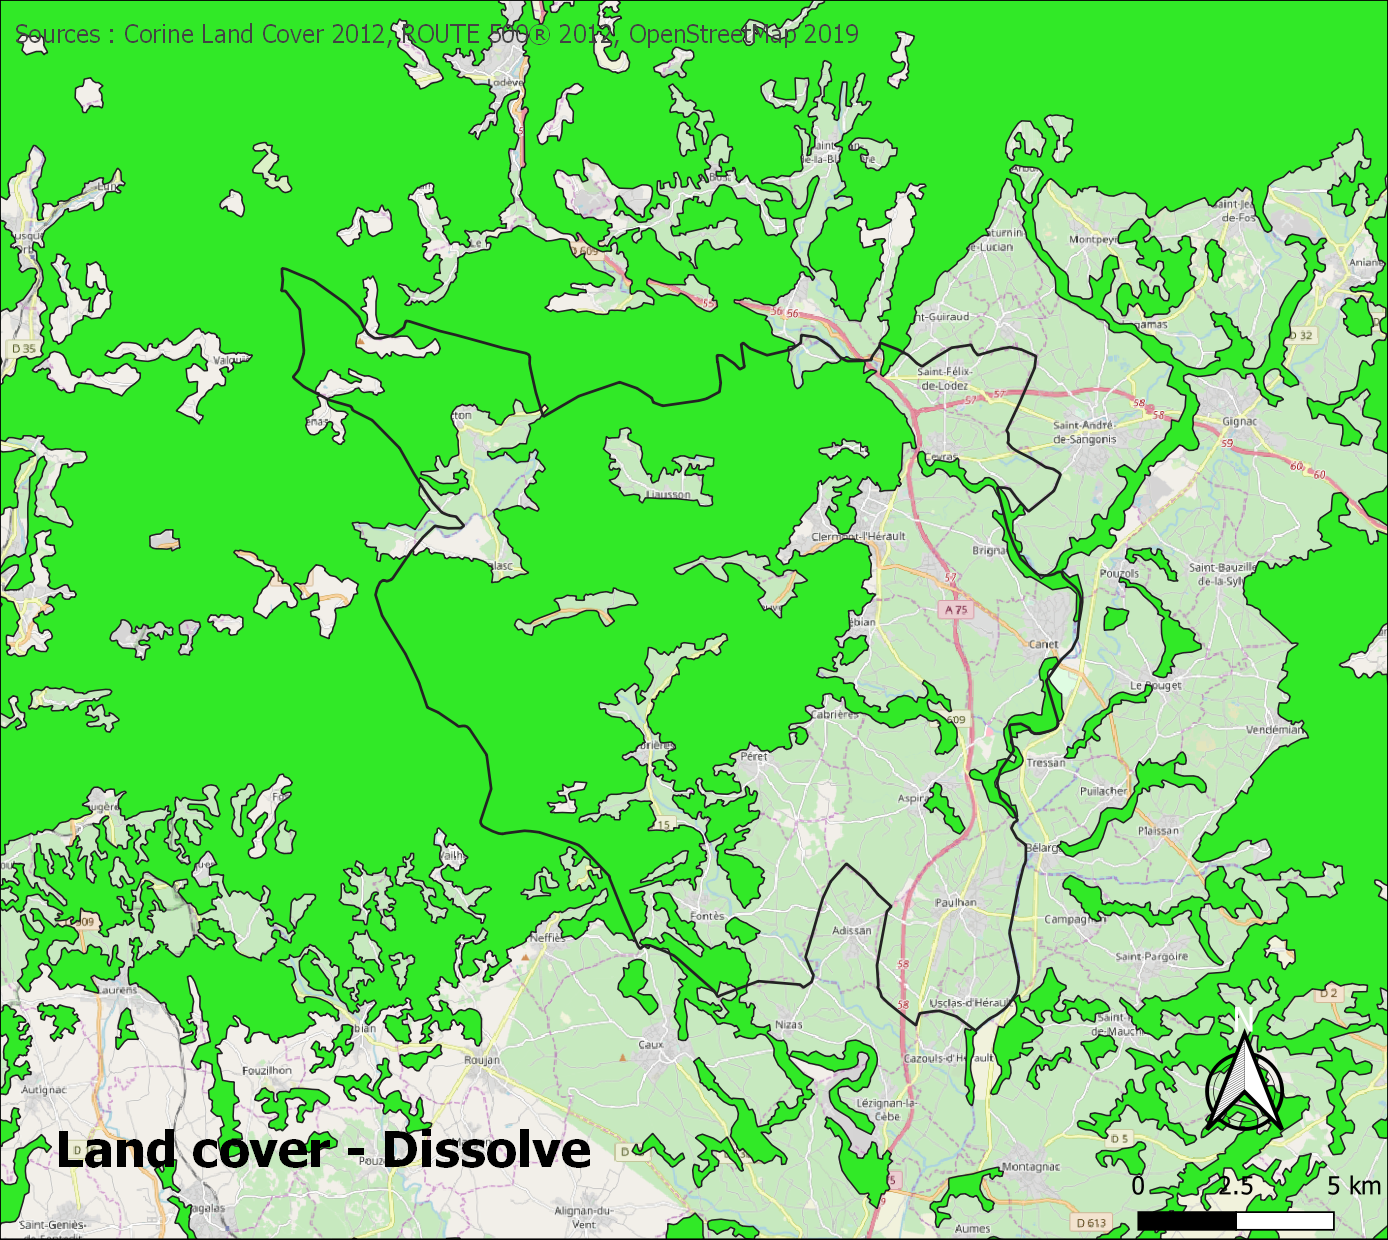
\includegraphics[width=\textwidth]{pictures/CBC/cbcLanduseDissolve.png}
      \caption{Étape 2}
   \end{subfigure}
   \begin{subfigure}[b]{.48\textwidth}
      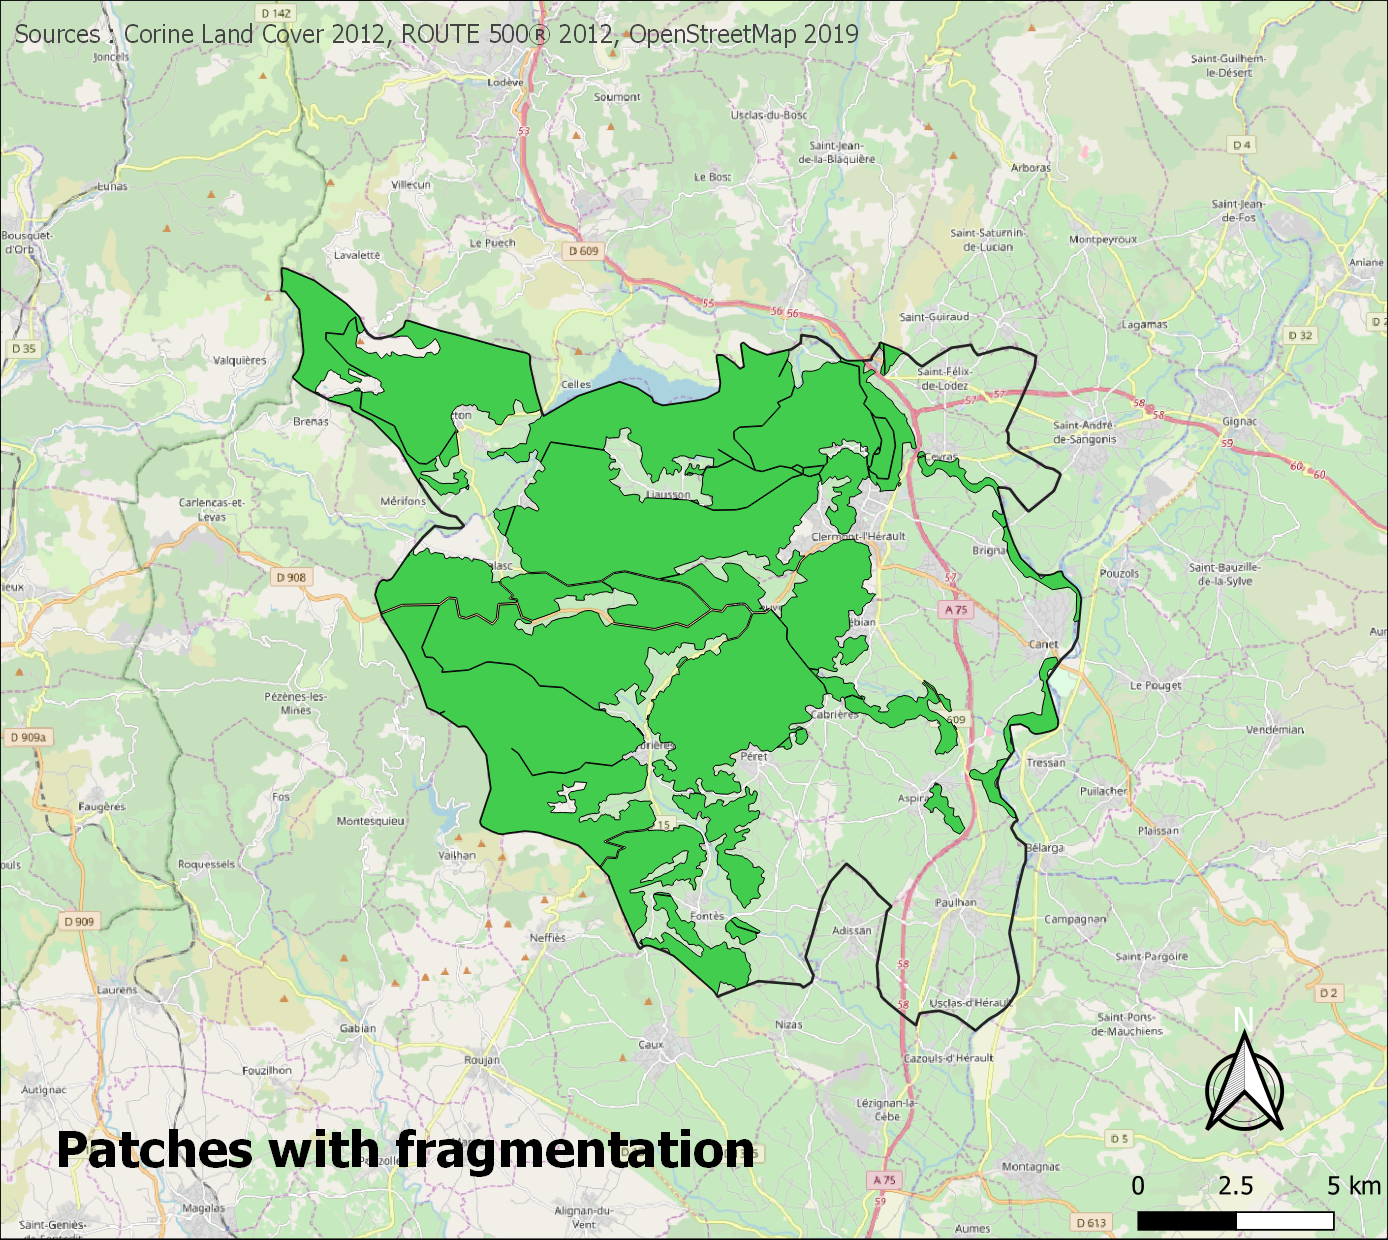
\includegraphics[width=\textwidth]{pictures/fragmPatches.png}
      %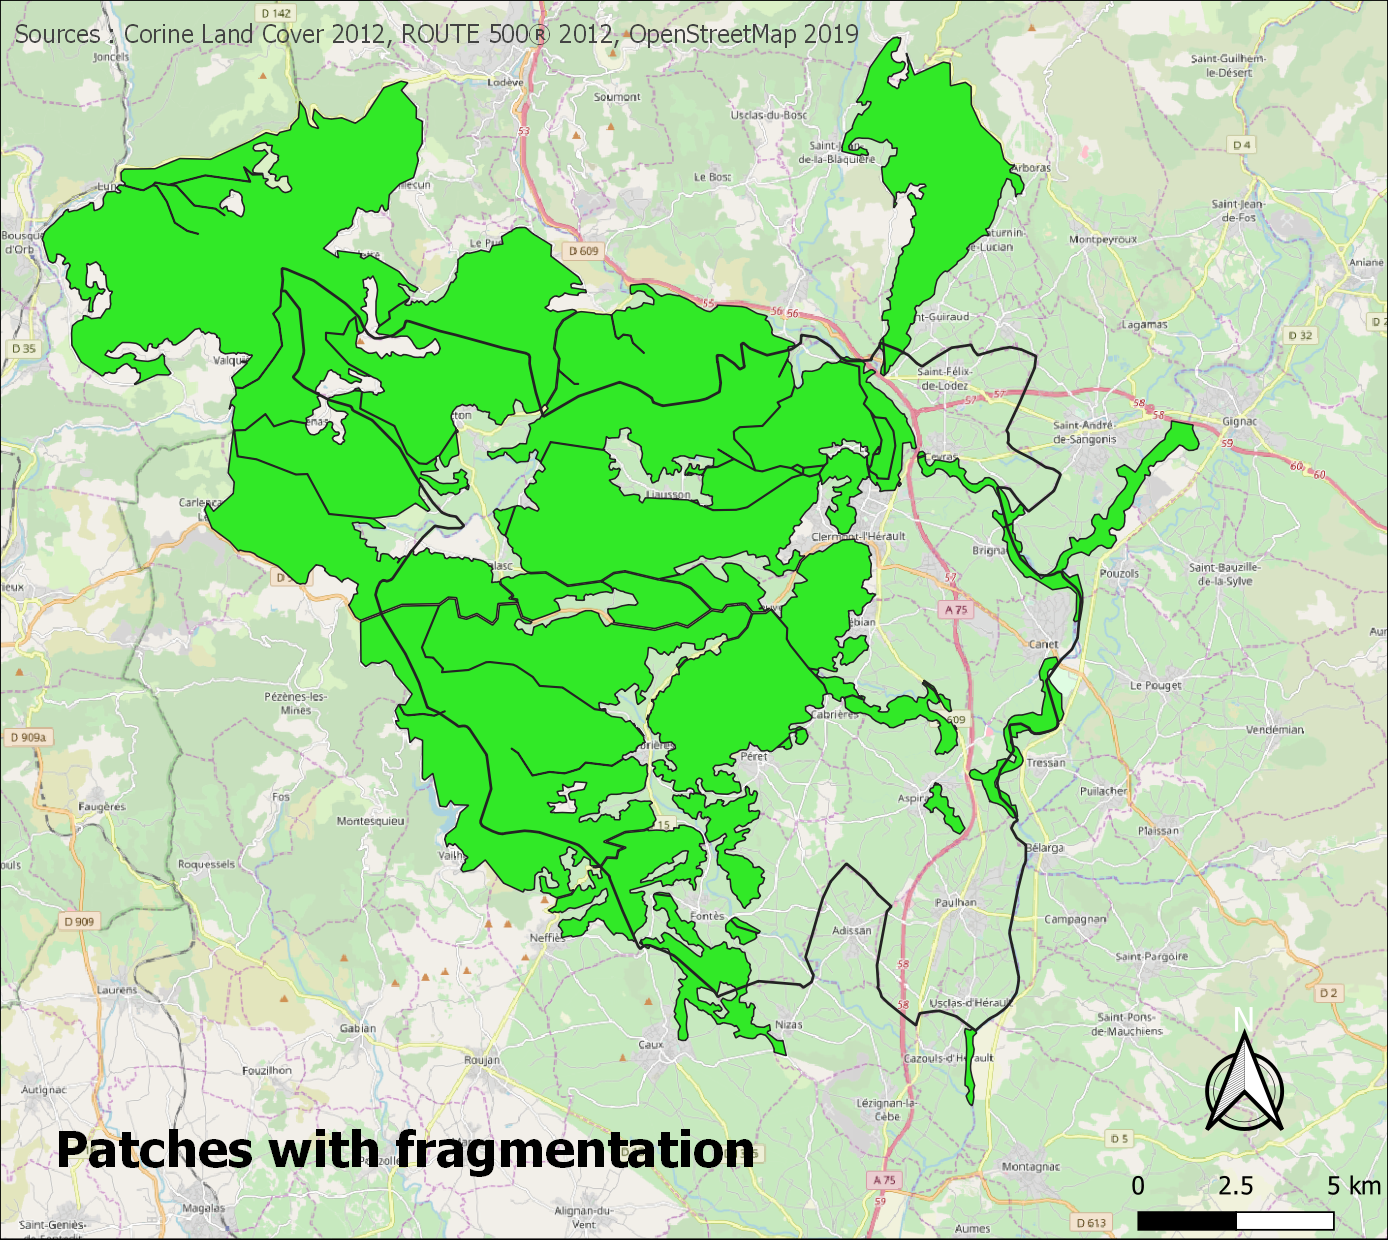
\includegraphics[width=\textwidth]{pictures/CBC/cbcFragmPatches.png}
      \caption{Étape 3}
   \end{subfigure}
   \begin{subfigure}[b]{.48\textwidth}
      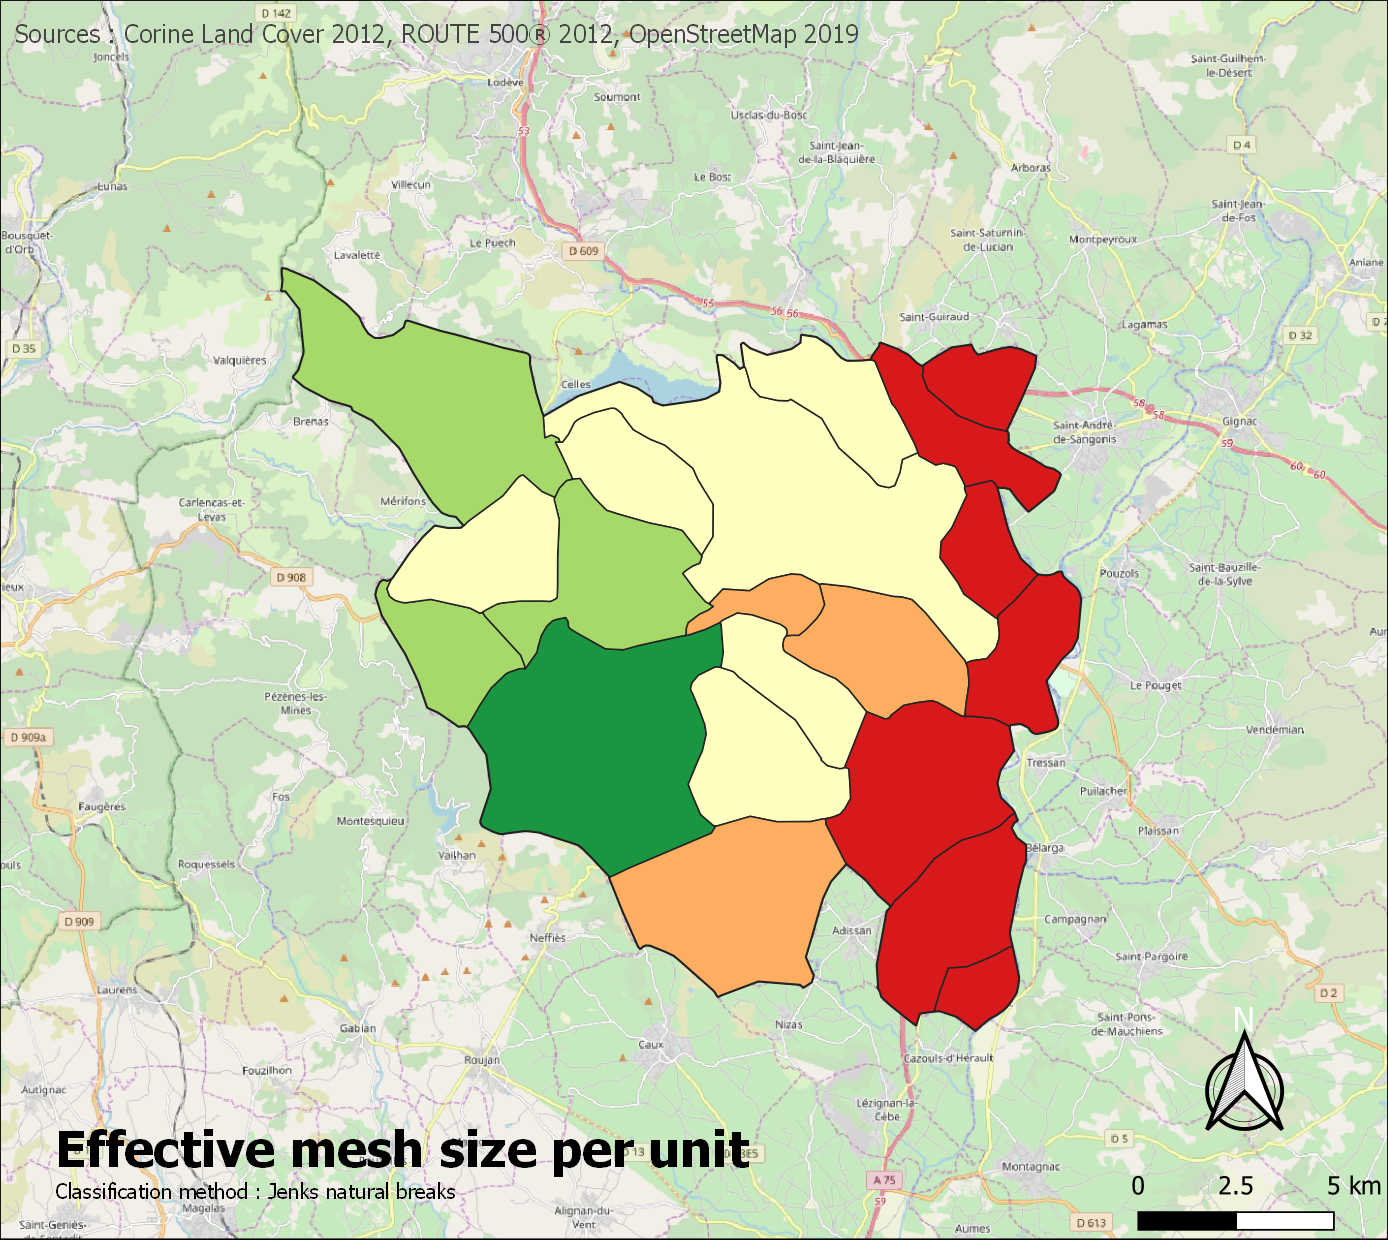
\includegraphics[width=\textwidth]{pictures/results.png}
      %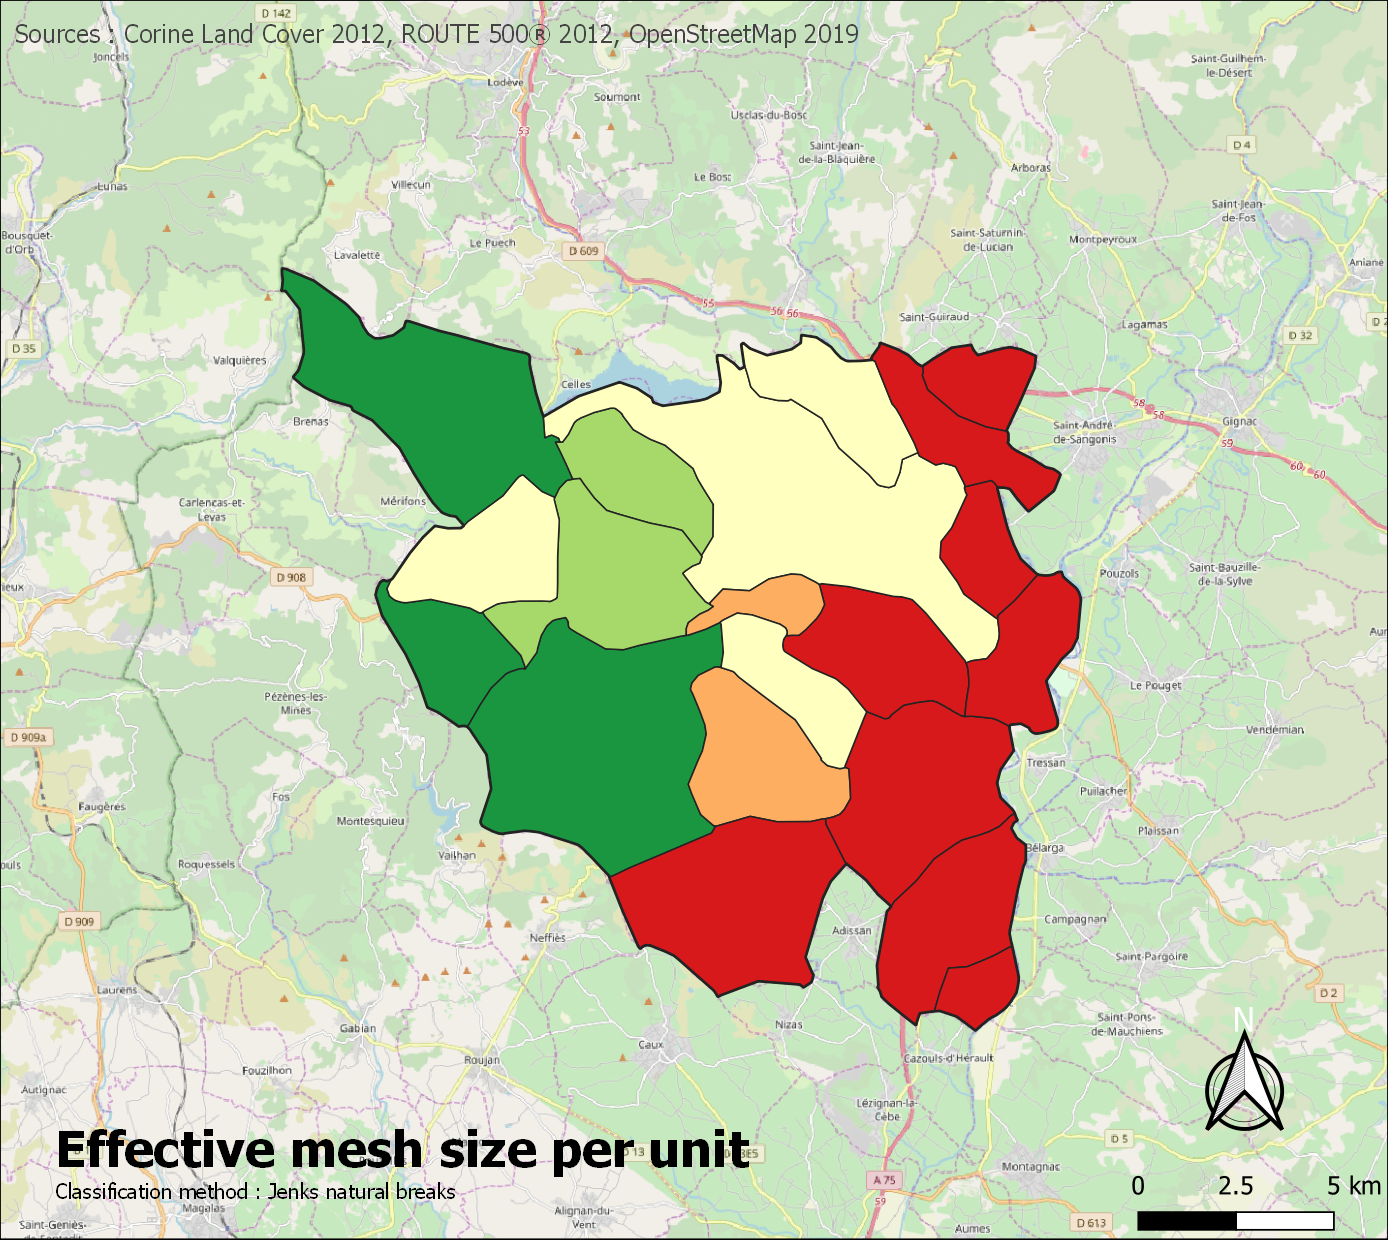
\includegraphics[width=\textwidth]{pictures/CBC/cbcResults.png}
      \caption{Étape 4}
   \end{subfigure}
   \caption{Cas d'utilisation de \tool\ : des données brutes à la taille effective de maille}
   \label{fig:usecase}
\end{figure}

La figure \ref{fig:usecase} montre l'occupation du sol initiale et le résultat de chaque étape.

Pour reproduire les résultats :
\begin{itemize}
    \item Copier le répertoire \texttt{sample\_data} localement
    \item Ouvrir \tool
    \item Choisir le dossier (\texttt{sample\_data/CUT}) comme dossier de travail
    \item Ouvrir le fichier de configuration \texttt{EPCI\_Clermontais\_2012\_CUT.xml} (icône   \includesvg[scale=0.6]{pictures/mActionFileOpen.svg})
    \item Vérifier que la configuration a été correctement chargée
    \item Lancer les étapes 2 puis 3 puis 4
\end{itemize}

%Legends are not automatically generated.



%\animategraphics[autoplay,loop,width=\textwidth,controls,scale=0.5]{1}{pictures/Image_}{1}{4}

\section{Pour aller plus loin...}

\subsection{Temps d'exécution}

Les temps d'exécution dépendent de l'emprise géographique du territoire d'étude et du volume de données sélectionnées. L'étape la plus longue est habituellement le regroupement des géométries en étape 2 ou le calcul de la différence en étape 3.

Un banc d'essai plus complet est actuellement en train d'être réalisé en utilisant des configuration plus ou moins complexes à des territoires de différentes échelles (Hérault, Languedoc-Roussillon, Occitanie et France entière).

À titre \textbf{purement indicatif} (les lancements ont été réalisés avec des configurations et des versions de \tool\ différentes), voici quelques temps d'exécution :

\begin{center}
\begin{tabular}{|c|ccc|}
    \hline
    Cas de test & Étape 1 & Étape 2 & Étape 3 \\
    \hline
    Languedoc-Roussillon & 40s & 137s & 72s \\
    Occitanie & 5mn25s & 11mn25s & 1mn54s \\
    France & 122h & 19h & 5h \\
    \hline
\end{tabular}
\end{center}


\subsection{Fichier de configuration}

La configuration est enregistrée dans un fichier XML et peut donc être ouverte dans un éditeur de texte. La figure \ref{fig:configFile} détaille le contenu du fichier de configuration \texttt{sample\_data/ECPI\_Clermontais\_2012/CBC/ECPI\_Clermontais\_2012\_CBC.xml}

\begin{figure}[h!]
    \centering
    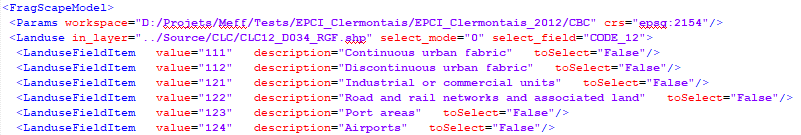
\includegraphics[scale=0.8]{pictures/configFile.png}
    \caption{Exemple de fichier de configuration}
    \label{fig:configFile}
    %\source{\tool\ v1.0}
\end{figure}

La balise \textit{Landuse} correspond à l'étape 2 et contient les attributs \textit{in\_layer} (couche d'entrée), \textit{select\_mode} ($0$ correspondant au mode de sélection \texttt{Par valeur de champ}) et \textit{select\_field} (champ de sélection de la couche d'entrée, ici \textit{CODE\_12}).
Pour chaque valeur de champ chargée, il existe une balise \textit{LanduseFieldItem} contenant les mêmes attributs que dans \tool\ (\textit{value}, \textit{description}, \textit{toSelect}).

Le fichier de configuration peut être édité manuellement si besoin, par exemple si les chemins relatifs doivent être adaptés à une nouvelle hiérarchie de fichier (\texttt{../Source} devenant \texttt{../../Source}). Éditer manuellement le fichier et le recharger dans \tool\ est alors plus simple que de changer les valeurs dans l'interface graphique.

%\subsection{Algorithms}

\subsection{Algorithmes}
\label{sec:algs}

\begin{minipage}[c]{.46\linewidth}
Les étapes de \tool\ sont implémentées comme des algorithmes $processing$ (disponibles dans la boîte à outils de traitements de \qgis). Comme le montre la figure \ref{fig:algs}, cinq algorithmes sont fournis :
\end{minipage} \hfill
\begin{minipage}[c]{.5\linewidth}
    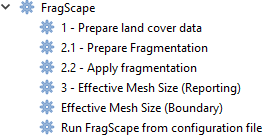
\includegraphics[scale=1]{pictures/algs.png}
    \captionof{figure}{Algorithmes de \tool}
    \label{fig:algs}
\end{minipage}


\begin{enumerate}
    \item \texttt{1 - Prepare land cover data} : correspond à l'étape 2. Sélection et regroupement des entités d'une couche d'occupation du sol. La sélection se fait à partir d'une expression (mode par valeur de champ non disponible).
    \item \texttt{2.1 - Prepare fragmentation data} : sélection et application d'une zone tampon à une couche contenant des éléments fragmentants pour modéliser leur empreinte au sol. Cet algorithme est exécuté pour chaque ligne de l'étape 3.
    \item \texttt{2.2 - Apply fragmentation} :  création d'une couche de patchs depuis la couche d'occupation du sol et les couches de fragmentation. Les couches de fragmentation sont fusionnées, la différence est calculée avec la couche d'occupation du sol et cette couche de différence est convertie en géométrie simple pour obtenir la couche de patchs. Cet algorithme est exécuté à la fin de l'étape 3.
    \item \texttt{3 - Effective mesh size (Reporting)}: calcul des indicateurs détaillés en section \ref{sec:metrics} depuis une couche de patchs pour chaque unité de la couche de rapportage d'après la méthode choisie (cf section \ref{sec:cbc}). Cet algorithme est appelé à l'étape 4 pour produire la couche de sortie.
    \item \texttt{Effective mesh size (Boundary)} : calcul des indicateurs de fragmentation comme l'algorithme précédent mais pour l'ensemble du territoire (la couche ne doit contenir qu'une entité). Cet algorithme est appelé à l'étape 4 pour chaque unité de rapportage et pour obtenir la taille effective de maille globale.
    \item \texttt{Run FragScape from configuration file} : exécution de la chaîne de traitements de \tool\ depuis un fichier de configuration. Cet algorithme peut être utilisé pour reproduire des résultats depuis une configuration déjà existante, lancer les traitements en arrière-plan ou pour exécuter toutes les étapes en un lancement.
\end{enumerate}




\section{FAQ}

\begin{itemize}
\item \textbf{Les champs ne sont pas chargés dans le widget \includesvg{pictures/mIconExpression.svg}, pourquoi ?} Si les champs n'apparaissent pas, c'est que la couche associée n'a pas été chargée même si elle apparaît dans la liste déroulante. Sélectionner une autre couche puis re-sélectionner la couche initiale.

\item \textbf{Quelle méthode dois-je utiliser, CUT ou CBC ?} La méthode CBC a été conçue pour répondre au biais dû à l'«effet frontière» et il est donc conseillé de l'utiliser. La méthode CUT est disponible pour permettre la comparaison avec d'ancien résultats ou si les frontières ne sont pas problématiques.

\item \textbf{Les éléments de fragmentation sont déjà inclus dans la couche d'occupation du sol, dois-je lancer l'étape 3 quand même ?} Dans \tool\ 1.0, la couche d'entrée des étapes 3 et 4 ne peut pas être directement sélectionnée et doit avoir été générée par \tool. Dans le cas où les éléments de fragmentation sont déjà inclus dans les données d'occupation du sol, il faut quand même lancer l'étape 3.

\item \textbf{Puis-je appliquer les traitements de \tool\ à une couche non produite par \tool\ ?} Pour appliquer un traitement spécifique de \tool\ à des données spécifiques, il est possible d'utiliser les algorithmes de \tool\ décrits en section \ref{sec:algs}.

\end{itemize}

\frameboxbegin{Bonnes pratiques}
\begin{itemize}
    \item Ne pas utiliser d'espaces ni de caractères spéciaux dans les noms de fichier.
    \item Ne pas utiliser de caractères spéciaux ni d'accents dans les valeurs de champ.
    \item Sauvegarder la configuration de \tool\ régulièrement.
    \item Vérifier le résultats de chaque étape.
    \item Si un bug inexpliqué survient, sauvegarder la configuration, quitter \tool\, relancer \tool\ et recharger la configuration sauvegardée. Si le bug persiste, quitter et relancer QGIS. Si le bug persiste toujours, contacter l'équipe de support.
\end{itemize}
\frameboxend

\subsection*{Messages d'erreur}

\begin{itemize}
    \item \textbf{\color{red}Layer XXX is already loaded in QGIS, please remove it.} \tool\ ne peut pas supprimer un fichier s'il est déjà chargé dans QGIS. Supprimer la couche XXX de QGIS et relancer le traitement \tool.
    \item \textbf{\color{red}The process cannot access the file because it is being used by another process: XXX.} Vérifier que le fichier XXX n'est pas utilisé par un autre programme. Si ce n'est pas le cas, quitter et relancer QGIS, relancer \tool, réouvrir le fichier de configuration et relancer le traitement \tool. Ce bug peut arriver notamment quand l'étape 3 est relancée après l'étape 4.
\end{itemize}

%\subsubsection*{}

\addcontentsline{toc}{section}{Bibliographie}
\printbibliography

\end{document}
